\subsection{Databse Implementation}
\label{sec:databaseImplementaion}
The final implemented databse architecture is displayed in figure \ref{fig:databaseImplementation}. The tables related to
the avatar: \code{AVATAR}, \code{AVATAR\_INVENTORIES}, \code{SHOP\_ITEMS} and \code{AVATAR\_ITEM\_SLOTS} are not used in the system because 
the avatar idea was put on hold. The rows \code{location\_latitude} and \code{location\_longtitude} in the table \code{CHILDREN} are also
not used because we did not implement updating the pollen feed based on current location.

The arrows symbolize relations, where the big end is the refereced key and the small end is the foreign key.

\begin{figure}
	\begin{center}
	\begin{sideways}
		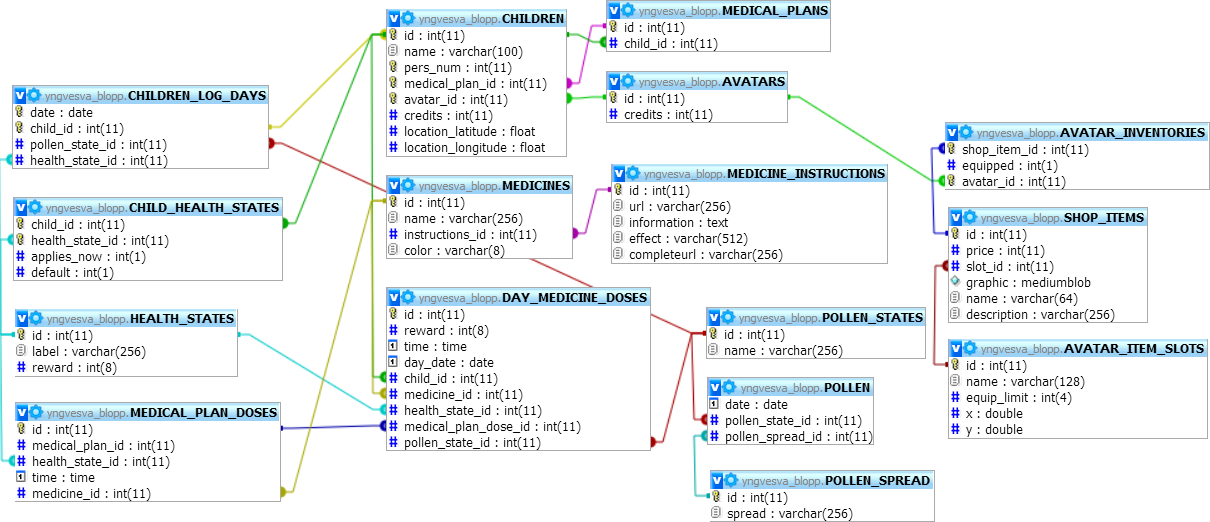
\includegraphics[width=0.8\paperheight]{Pictures/ArchPictures/DatabaseImplementation}
	\end{sideways}
	\end{center}
	\caption{Implemented Database Architecture}
	\label{fig:databaseImplementation}
\end{figure}